\section{Gustavo}

\setbeamertemplate{caption}{\raggedright\insertcaption\par}
\begin{frame}{Introduction}{Gustavo S. Buschle\newline<gbusch14@student.aau.dk>}
	\begin{figure}[h!]
		%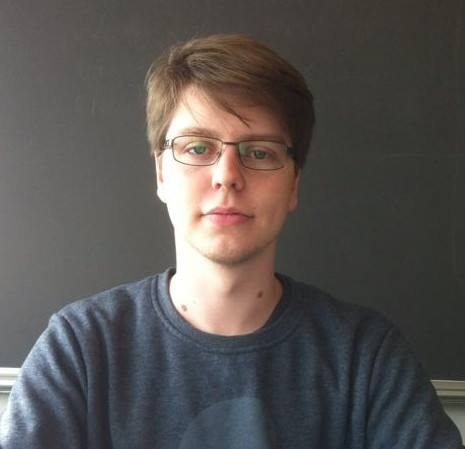
\includegraphics[width=0.3\textwidth]{images/gustavo.jpg}
		\caption{Gustavo S. Buschle}
		\centering    		
	\end{figure}
\end{frame}
\setbeamertemplate{caption}[default]

%intro to laser
%    "our other module is ..." segue from anthony
%    How we assembled the parts (case,slipring,etc which anthony mentions)
%    (pics)
%    two versions of laser
%        v1arduino: hard to sync
%        v2non-ard: slow
%
%ROS
%    learning curve
%    ROS compoenets we used
%
%Slam (make sure not to talk over emil)
%    add pics
%    didn't work very well
%
%(linux clock problems?)
